\begin{figure}[!htbp]
\centering
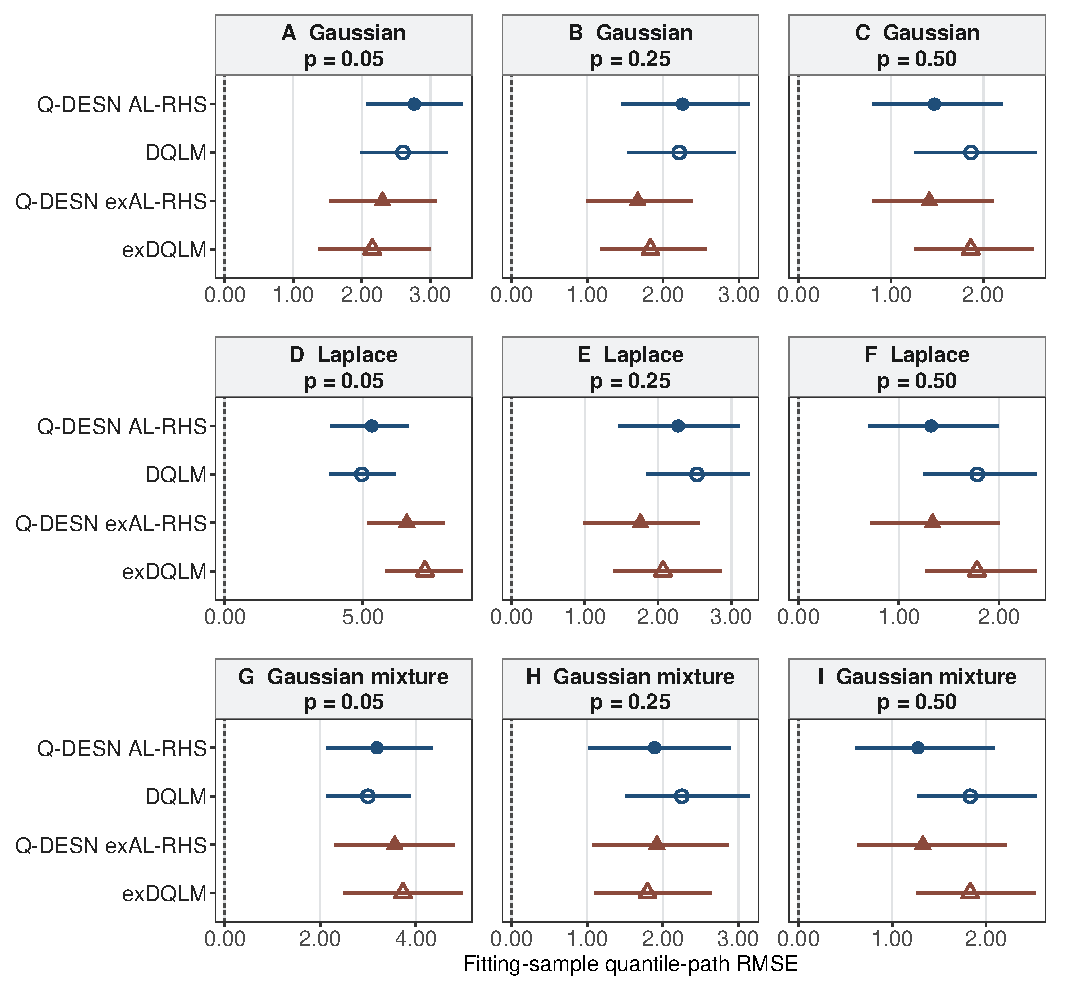
\includegraphics[width=0.98\textwidth]{figures/independent_simulation/qdesn_pro_review_mcmc_fit_rmse.pdf}
\caption{MCMC fitting-sample recovery in the single-quantile study. Points and equal-tailed 95\% intervals summarize draw-wise quantile-path root mean squared error (RMSE); lower values are better. Navy circles identify \(\AL\) models and muted-brick triangles \(\exAL\) models; filled symbols denote Q--DESN and open symbols their dynamic linear comparators. Panels A--I identify the observation-error family and probability level, with separate horizontal scales. The dashed line marks exact recovery. The summaries condition on the simulated series and the criterion-specific specification.}
\figalt{Nine panels compare posterior fitting-sample quantile-path RMSE means
and 95 percent intervals for four models across three observation-error families and
three probability levels. Lower values are better.}
\label{fig:simulation-500obs-mcmc-fit-rmse-intervals}
\end{figure}
